\section{Analysis}
\label{sec:analysis}

\begin{figure*}
%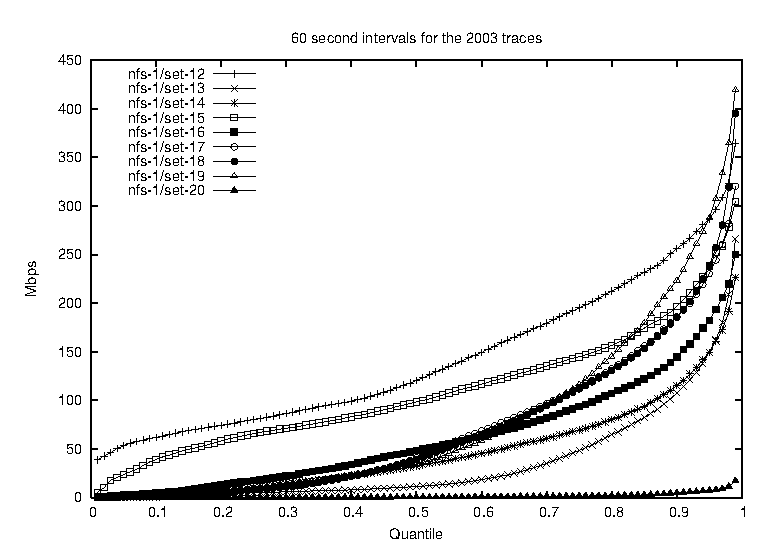
\epsfig{width=2.1in, angle=0, file=graphs/Mbps-nfs-1.ps}
%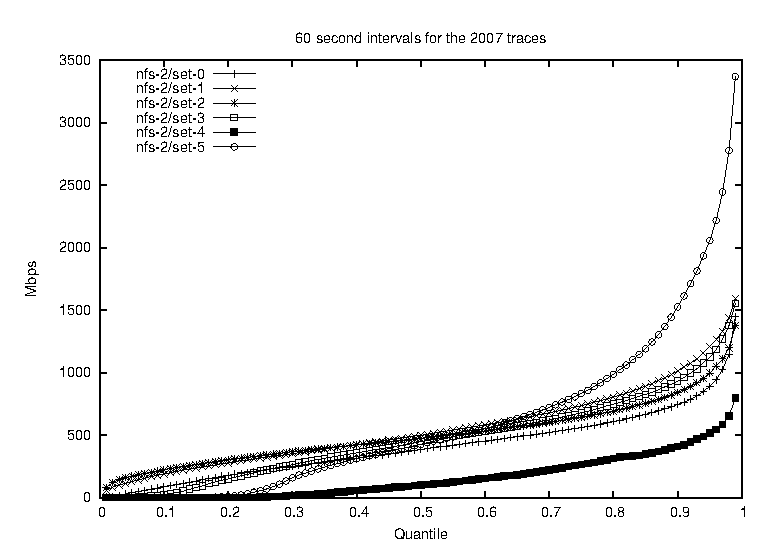
\epsfig{width=3.2in, angle=0, file=graphs/Mbps-nfs-2.ps}
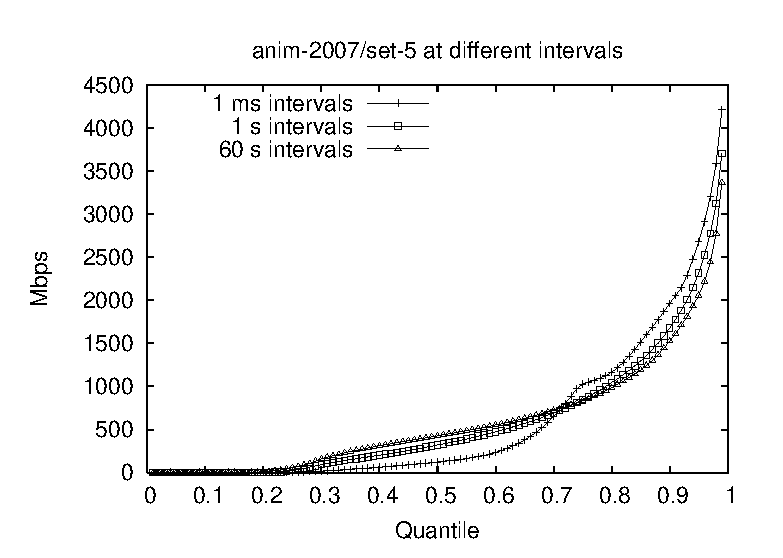
\epsfig{width=3.3in, angle=0, file=graphs/Mbps-nfs-2-set-5.ps}
\epsfig{width=3.3in, angle=0, file=graphs/Mbps-tails.ps}
\vspace{-0.2in}
\caption{Bandwidth measured in the collection process.  In Figure (b),
anim-2007/set-5 at different intervals is the top group of 4 lines, and
anim-2003/set-12 is the bottom group of 4 lines. With 60s intervals, 
anim-2003/set-12 does not show the 0.9999 quantile 
because there were insufficient data points.}
\label{fig:bwrolling-mbps}
\end{figure*}


% nfs_hostinfo_rates, nfs_hostinfo_rate_quantiles, nfs_hostinfo_cube;
% choose sets nfs-2/set-[2,5]; nfs-1/set-[5,12]
%                     03+10, 06+13 ; 20+42, 27+49

% select from_unixtime(group_time), group_count/3600 where dataset = 'nfs-1/set-12' and group_time is not null and host is null  and operation is null and direction is null and op_dir is null
% nfs-1/set-5: 2003-09-16 .. 2003-09-18
% nfs-1/set-12: 2003-12-09 - 2003-12-10
% nfs-2/set-2: 2007-03-05 .. 2007-03-11
% nfs-2/set-5: 2007-10-12 .. 2007-10-17
% from hostinfo.hg + a few minor tweaks (n/a) for set-5 readdirplus
\begin{table*}\begin{center}
\begin{tabular}{|r||r|r||r|r||r|r||r|r|}
\hline
  & \multicolumn{2}{c||}{anim-2003/set-12} & \multicolumn{2}{c||}{anim-2003/set-5} & \multicolumn{2}{c||}{anim-2007/set-2} & \multicolumn{2}{c|}{anim-2007/set-5} \\
   operation &   Mops & bytes/op &   Mops & bytes/op &   Mops & bytes/op &   Mops & bytes/op \\
\hline
%     symlink &     0.008 &   201 &     0.000 &    92 &     0.001 &   415 &     0.000 &   458 \\
%       rmdir &     0.204 &   152 &     0.001 &    64 &     0.020 &   167 &     0.002 &   178 \\
%       mkdir &     0.173 &   304 &     0.005 &   193 &     0.071 &   336 &     0.004 &   334 \\
%      rename &     0.028 &   270 &     0.002 &   150 &     0.250 &   367 &     0.055 &   348 \\
%\hline
%      fsinfo &     0.023 &   176 &     0.003 &    72 &     1.352 &   176 &     0.619 &   176 \\
%        link &     0.000 &    86 &     0.000 &    88 &     3.259 &   314 &     0.182 &   322 \\
%        null &     0.259 &     5 &     0.087 &     4 &     1.482 &     4 &     2.808 &     4 \\
%      create &     0.296 &   295 &     0.965 &   200 &     4.639 &   367 &     1.616 &   344 \\
%\hline
%      remove &     0.275 &   136 &     0.641 &    69 &     8.419 &   194 &     1.500 &   186 \\
%     setattr &     0.716 &   133 &     1.075 &   136 &     9.415 &   193 &     6.531 &   192 \\
     readdir &     4.579 &   281 &     1.132 &  3940 &    28.318 &  4089 &    18.350 &  4071 \\
 readdirplus &     0.632 &  2307 &     0.000 &  n/a  &    32.806 &  1890 &    20.271 &  2001 \\
    readlink &     0.081 &    74 &     0.049 &    79 &    25.421 &   204 &    42.335 &   203 \\
      fsstat &    19.875 &    56 &    50.416 &    56 &     0.017 &   180 &     0.003 &   180 \\
       write &    14.546 &  9637 &    30.236 &  7880 &    32.390 & 13562 &    45.177 & 15015 \\
\hline
      lookup &   134.108 &    83 &    82.823 &    92 &   643.854 &   239 &   807.127 &   235 \\
        read &   345.743 &  1231 &   165.969 &  7855 &  1460.669 & 14658 &  1761.199 & 12301 \\
      access &     1.858 &   136 &     0.000 &   136 &  4000.204 &   136 &  3570.404 &   136 \\
     getattr &   244.650 &   104 &   967.961 &   104 &  6598.515 &   124 &  2756.785 &   123 \\
\hline
 {\bf total} &   768.053 &   790 &  1301.364 &  1274 & 12851.102 &  1833 &  9034.968 &  2599 \\
\hline
\end{tabular}\end{center}
\vspace{-0.15in}
\caption{symlink, rmdir, mkdir, and rename were pruned as there were
fewer than 1 million operations; fsinfo, link, null, create, remove,
and setattr were pruned as there were fewer than 10 million
operations.  The Mops column could be calculated from nfsstat, but the
bytes/op column could not.}

\label{table:nfs-stats-overview}
\end{table*}


% LocalWords:  nfs hostinfo unixtime op dir hg readdirplus anim symlink rmdir
% LocalWords:  mkdir fsinfo setattr readdir readlink fsstat getattr nfsstat

\begin{figure*}
% 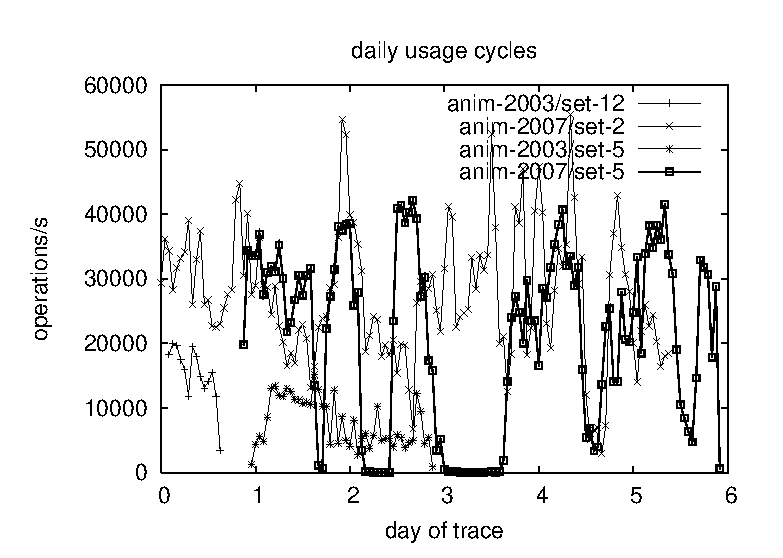
\epsfig{width=2.1in, angle=0, file=graphs/daily-oprate.ps}
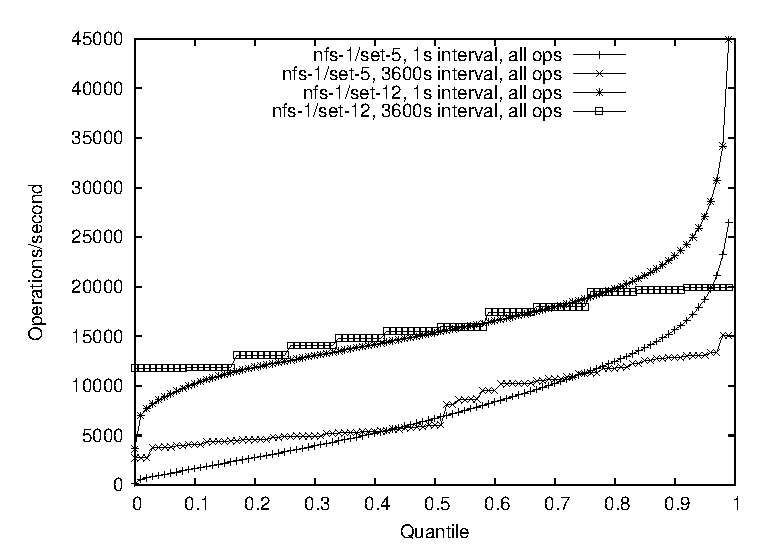
\epsfig{width=3.3in, angle=0, file=graphs/allops-quantile-nfs-1.ps}
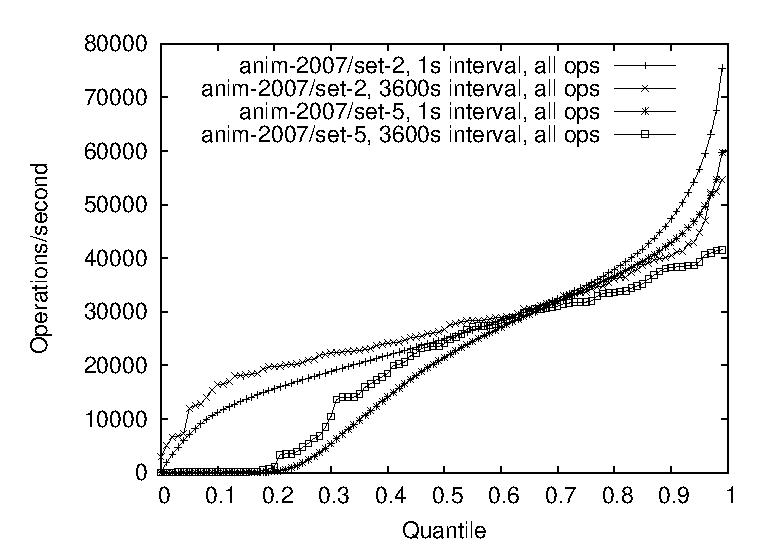
\epsfig{width=3.3in, angle=0, file=graphs/allops-quantile-nfs-2.ps}
\vspace{-0.2in}
\caption{Operation rates, as quantiles, for anim-2003, anim-2007.}
\label{fig:oprates}
\end{figure*}


% LocalWords:  anim


Analyzing very large traces can take a long time.  While our custom
binary format enables efficient analysis, and our analysis techniques
are efficient, it can still take 4-8 hours to analyze a single set of
the 2007 traces.  In practice, we analyze the traces in parallel on a
small cluster of four core 2.4GHz Opterons.  Our analysis typically
becomes bottle-necked on the file servers that serve up to 200MiB/s each
once an analysis is running on more than 20 machines.

We collected data at two times: August 2003 - February 2004 (anim-2003), and January 2007 - October 2007
(anim-2007).  We collected data using a variety of mirror
ports within the company's network.
The network design is
straightforward: there is a redundant set of core routers, an
optional mid-tier of switches to increase the effective port count of
the core, and then a collection of edge switches that each cover one
or two racks of rendering machines.  Most of our traces were taken by
mirroring links between rendering machines and the rest of the network.
For each collected dataset, we would start the collection
process, and let it run either until we ran out of disk space, or we
had collected all the data we wanted.  Each of these runs comprises a
set.  We have 21 sets from 2003, and 8 sets from 2007. 

We selected a subset of the data to present, two datasets from 2003
and two from 2007.  The sets were selected both because they are
representative of the more intensive traces from both years, and to
show some variety in the data.  We identified clients as hosts that
sent requests, servers as hosts that sent replies, and caches as hosts
that acted as both clients and servers. Further information on each
dataset can be found on the trace download
page~\cite{animation-bear-traces}.

\begin{itemize}
\item{anim-2003/set-5}: A trace of 79 clients accessing 50 NFS servers.  
NFS caches are seen as servers in this trace.

\item{anim-2003/set-12}: A trace of 1634 clients accessing 1 NFS
server.  NFS caches are seen as clients in this trace.

\item{anim-2007/set-2}: A trace of 273 clients accessing 40 NFS
servers at the same site as anim-2003/set-5.  The other traces of
clients at this site are similar to set-2.

\item{anim-2007/set-5}: A trace of 135 clients accessing 50 NFS
servers, and 8 caches acting as both clients and servers, although
because of the port mirroring setup, we did not see some of the
responses from the caches.  This trace is at a different site from
set-2 and shows higher burstiness.
% See graphs/hostinfo.hg for more on asymmetric packet capture
\end{itemize}

\subsection{Capture performance}

We start our analysis by looking at the performance of our capture
tool.  This validates our claims that we can capture packets at very
high data rates.  We examine the capture rate of the tool by
calculating the megabits/s (Mbps) and kilo-packets/s (kpps) for
20 overlapping sub-intervals of a specified length.  For example if our
interval length is 60 seconds, then we will calculate the bandwidth
for the interval 0s-60s, 3s-63s, 6s-66s, ... end-of-trace.  We chose
to calculate the bandwidth for overlapping intervals so that we would not
incorrectly measure the peaks and valleys of cyclic patterns aligned to the interval length.
We use the approximate quantile so we can summarize results with billions of
underlying data points.  For example, we
have 11.6 billion measurements for anim-2007/set-0 at a 1ms interval
length.  This corresponds to the 6.7 days of that trace.
% 11.6 * 10^9 * 0.001 / 20 = 580,000 / 86400 = 6.7

Figure~\ref{fig:bwrolling-mbps}(a) shows anim-2007/set-5 at
different interval lengths.  This graph shows the effectiveness of our
tracing technology, as we have sustained intervals above 3Gb/s
(358MiB/s), and 1ms intervals above 4Gb/s (476MiB/s). Indeed these
traces show the requirement for high speed tracing, as 5-20\% of the
trace intervals have sustained intervals above 1Gbit, which is above
the rate at which Leung~\cite{LeungUsenix08} noted their tracing tool
started to drop packets.  The other sets from anim-2007 are somewhat
less bursty, and the anim-2003 data shows much lower peaks because of
our more limited tracing tools, and a wider variety of shapes, because
we traced at more points in the network.

Figure~\ref{fig:bwrolling-mbps}(a) also emphasizes how bursty the traffic was
during this trace. While 50\% of the intervals were above 500Mbit/s for
60s intervals, only 30\% of the intervals were above 500Mbit/s for 1ms
intervals.  This burstiness is expected given that
general Ethernet and filesystem
traffic have been shown to be
self-similar~\cite{Gribble98selfsimilar,Leland94selfsimilar}, which implies the network traffic is also bursty.
It does make it clear that we need to look at short time intervals in
order to get an accurate view of the data.

Figure~\ref{fig:bwrolling-mbps}(b) shows the tail of the distributions for
the capture rates for two of the trace sets.  The relative similarity
between the Mbps and kpps graphs is simply because packet size
distributions are relatively constant.  The traces show the remarkably high
burstiness of the 2007 traces.  While 90\% of the 1ms intervals are
below 2Gb/s, 0.1\% are above 6Gb/s.  We expect we would have seen
slightly higher rates, but because of our configuration error for the
2007 capture tool, we could not capture above about 8Gb/s.

% \begin{figure*}
% 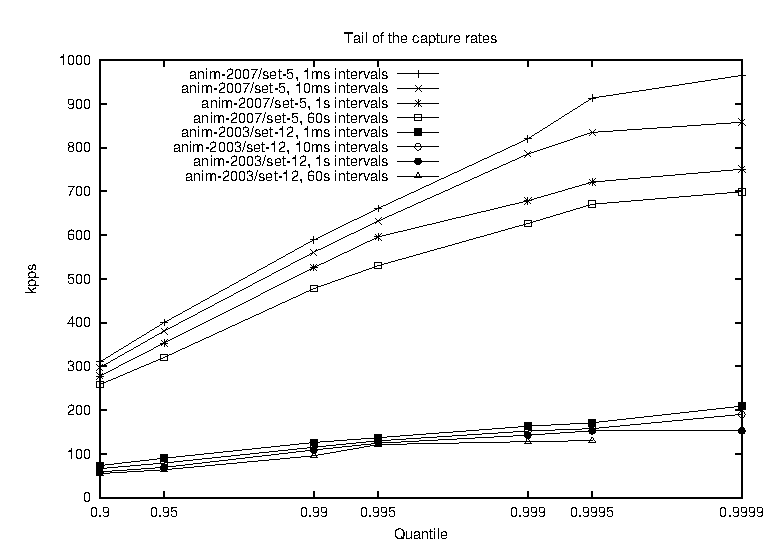
\epsfig{width=2.1in, angle=0, file=graphs/kpps-tails.ps}
% \caption{Tail of the quantiles in Mbps and kpps for the anim-2007 traces.}
% \label{fig:capture-tails}
% \end{figure*}

\subsection{Basic NFS analysis}

\begin{figure}
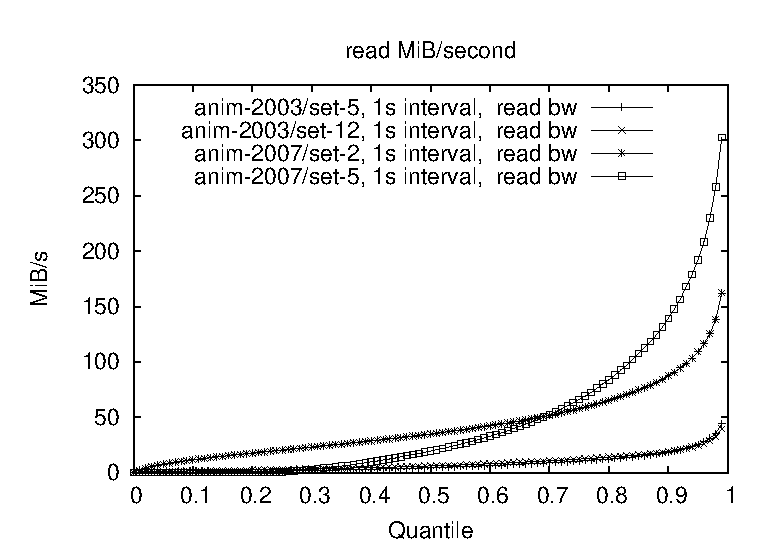
\epsfig{width=3.2in, angle=0, file=graphs/bw-read.ps}
%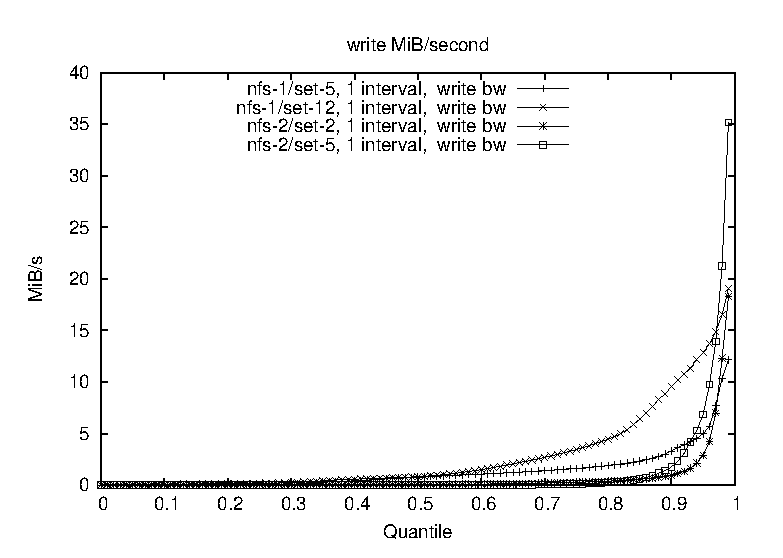
\epsfig{width=2.1in, angle=0, file=graphs/bw-write.ps}
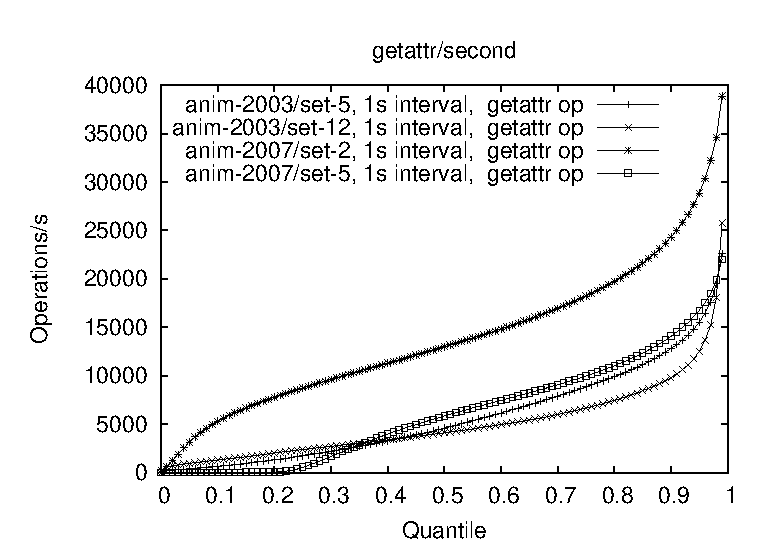
\epsfig{width=3.2in, angle=0, file=graphs/ops-getattr.ps}
\vspace{-0.1in}
\caption{Bandwidth for reads and operation rate for getattrs in the four traces.}
\label{fig:bw-ops-quantiles}
\end{figure}

Examining the overall set of operations used by a workload provides
insight into what operations need to be optimized to support the
workload.  Examining the distribution of rates for the workload tells
us if the workload is bursty, and hence we need to handle a higher
rate than would be implied by mean arrival rates, and if there are
periods of idleness that could be exploited.

Table~\ref{table:nfs-stats-overview} provides an overview of all the
operations that occurred in the four traces we are examining in more
detail.  It shows a number of substantial changes in the workload
presented to the NFS subsystem.  First, the read and write sizes have
almost doubled from the anim-2003 to anim-2007 datasets.  This trend is expected,
because the company moved from NFSv2 to NFSv3 between the two
tracing periods, and set the v3 read/write size to 16KiB.  The company told
us they set it to that size based on performance
measurements of sequential I/O.  The NFS version switch also accounts
for the increase in access calls (new in v3), and readdirplus (also
new in v3).  

We also see that this workload is incredibly read-heavy.  This is
expected; the animation workload reads a very large number of
textures, models, etc. to produce a relatively small output frame.
However, we believe that our traces under-estimate the number of write
operations.  We discuss the write operation underestimation below.
The abnormally low read size for set-12 occurred because
that server was handling a large number of stale filehandle requests.  The
replies were therefore small and pulled down the bytes/operation.  We
see a lot more getattr operations in set-5 than set-12 because set-12
is a server behind several NFS-caches, whereas set-5 is the workload
before the NFS-caches.

% select dataset, group_seconds, operations_per_second from xnfs_hostinfo_rate_quantiles where host is null and direction = 'send' and operation is null and op_dir is null and quantile = 0.99
\begin{table}
\begin{center}
\begin{tabular}{|l|r|r|r|}
\hline
dataset & 1s ops/s & 3600s ops/s & ratio \\
\hline
anim-2003/set-5  & 26,445 & 15,110 & 1.75$\times$ \\
anim-2003/set-12 & 44,926 & 19,923 & 2.25$\times$ \\
anim-2007/set-2  & 75,457 & 54,657 & 1.38$\times$ \\
anim-2007/set-5  & 59,727 & 41,550 & 1.44$\times$ \\
\hline
\end{tabular}
\end{center}
\vspace{-0.1in}
\caption{Operation rate ratios}
\label{table:99quant-differences}
\end{table}

% LocalWords:  xnfs hostinfo op dir ops anim


Table~\ref{table:99quant-differences} and
Figures~\ref{fig:oprates}(a,b) show how long averaging intervals can
distort the load placed on the storage system.  If we were to develop
a storage system for the hourly loads reported in most papers, we
would fail to support the substantially higher near peak (99\%) loads
seen in the data.  It also hides periods of idleness that could be
used for incremental scrubbing and data reorganization.  We do not
include the traditional graph of ops/s vs.\ time because our workload
does not show a strong daily cycle.  Animators submit large batches of
jobs in the evening that keep the cluster busy until morning, and
keep the cluster busy during the day submitting additional jobs.
Since the jobs are very similar, we see no traditional diurnal pattern
in the NFS load, although we do see the load go to zero by the end of
the weekend.

Figure~\ref{fig:bw-ops-quantiles} shows the read operation MiB/s and
the getattr operations/s.  It shows that relative to the amount of
data being transferred, the number of getattrs has been reduced,
likely a result of the transition from NFSv2 to NFSv3.  The graph
shows the payload data transferred, so it includes the offset and
filehandle of the read request, and the size and data in the reply,
but does not include IP headers or NFS RPC headers.  It shows that the
NFS system is driven heavily, but not excessively. The write operations/s graph
(not shown for space reasons) implies that the write bandwidth has
gotten more bursty, but has stayed roughly constant.

This result led us to further analyze the data.  We were surprised
that write bandwidth did not increase, even though it is not
implausible, as the frame output size has not increased.  We analyzed
the traces to look for missing operations in the sequence of
transaction ids, automatically inferring if the client is using a
big-endian or little-endian counter.  The initial results looked quite
good: anim-2007/set-2 showed 99.7\% of the operations were in sequence,
anim-2007/set-5 showed 98.4\%, and counting the skips of 128 transactions
or less, we found only 0.21\% and 0.50\% respectively (the remaining
entries were duplicates or ones that we could not positively tell if
they were in sequence or a skip).  However, when we looked one level
deeper at the operation that preceded a skip in the sequence, we found
that 95\% of the skips followed a write operation for set-2, and 45\%
for set-5.  The skips in set-2 could increase the write workload by a
factor of 1.5$\times$ if all missing skips after writes are associated with
writes.  We expected a fair number of skips for set-5 since we
experienced packet loss under load, but we did not expect it for
set-2. 

Further examination indicated that the problem came about because we
followed the same parsing technique for TCP packets as was used in
nfsdump2~\cite{ellardTraces}.  We started at the beginning of the
packet and parsed all of the RPCs that we found that matched all
required bits to be RPCs.  Unfortunately, over TCP, two back to back
writes will not align the second write RPC with the packet header, and
we will miss subsequent operations until they re-align with the packet
start.  While the fraction of missing operations is small, they are
biased toward writes requests and read replies. Since we had saved
IP-level trace information as well as NFS-level, we could write an
analysis that conservatively calculated the bytes of IP packets that
were not associated with an NFS request or reply.  Counting a
direction of a connection if it transfers over $10^6$ bytes, we found
for anim-2007/set-2 that we can account for $>$90\% of the bytes for
87\% of the connections, and for anim-2007/set-5 that we can account
for $>$90\% of the bytes for $>$70\% of the connections.  The greater
preponderance of missing bytes relative to missing operations
reinforces our analysis above that the losses are due to non-aligned
RPC's since we are missing very few operations, but many more bytes,
and reads and writes have a high byte to operation ratio.

While this supports our lesson that retaining lower level information
is valuable, this analysis also leads us to another one of our lessons:
extensive validation of the conversion tool is important.  Both
validation through validation statistics, and through the use of a
known workload that exercises the capture tools.  An NFS replay
tool~\cite{NingningFast05} could be used to generate a workload, the
replayed workload could be captured, and the capture could be compared
to the original replayed workload.  This comparison has been done to
validate a block based replay tool~\cite{AndersonFast04}, but has not
been done to validate an NFS tracing tool, as the work has simply assumed
tracing was correct.
% We can therefore use
% the timing information from requests and replies to identify gaps in
% the dataset and determine how many bytes were skipped.  This will
% allow us to approximate the number of missing writes.  Preservation of
% lower level information is a lesson we got right, and it will allow us
% to partially reconstruct flaws in the traces.  
We believe a similar
flaw is present in earlier traces~\cite{ellardTraces} because the same
parsing technique was used, although we do not know how much those traces were
affected.

\subsection{File sizes}

\begin{figure}
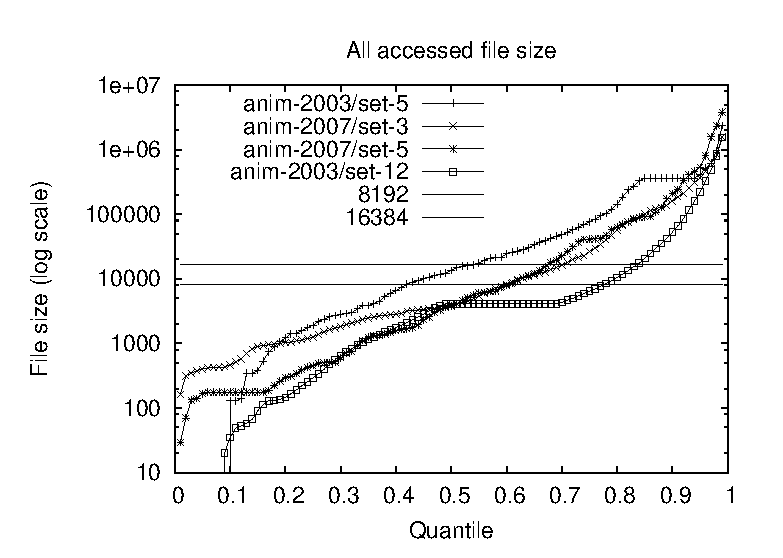
\epsfig{width=3.2in, angle=0, file=graphs/file-size.ps}
\vspace{-0.2in}
\caption{File size distribution for all accessed files.}
\label{fig:file-size}
\end{figure}

File sizes affect the potential internal fragmentation for a
filesystem.  They affect the maximum size of I/Os that can be
executed, and they affect the potential sequentiality in a workload.

Figure~\ref{fig:file-size} shows the size of files accessed in our
traces.  It shows that most files are small enough to be read in a single I/O: 
40-80\% of the files are smaller than 8KiB (NFSv2 read size) 
for the 2003 traces, and  70\% of the
files are smaller than 16KiB for the 2007 traces.
While there are larger files in the traces, 99\% of
the files are smaller than 10MiB.  The small file sizes present in this
workload, and the preponderance of reads suggest that a flash file
system~\cite{Kawaguchi95aflash-memory} or MEMS file
system~\cite{SchlosserFast04} could support a substantial portion of
the workload.

\subsection{Sequentiality}

\begin{figure}
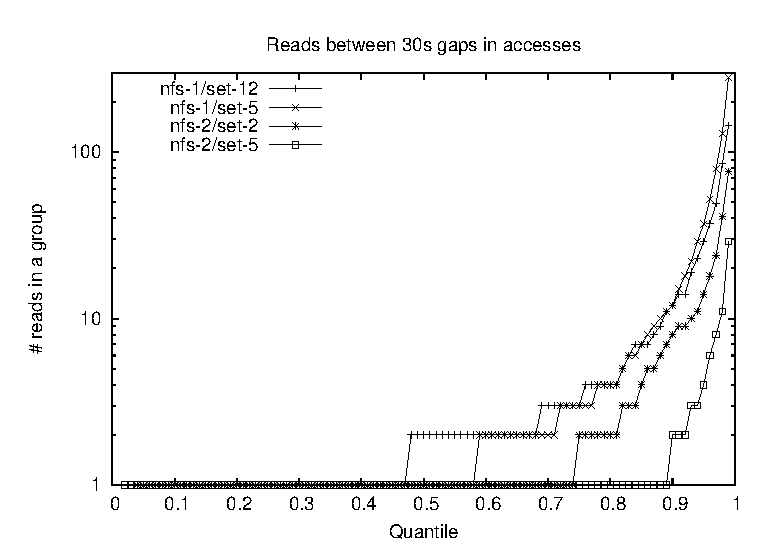
\epsfig{width=3.2in, angle=0, file=graphs/seq-read-group-counts.ps}
% 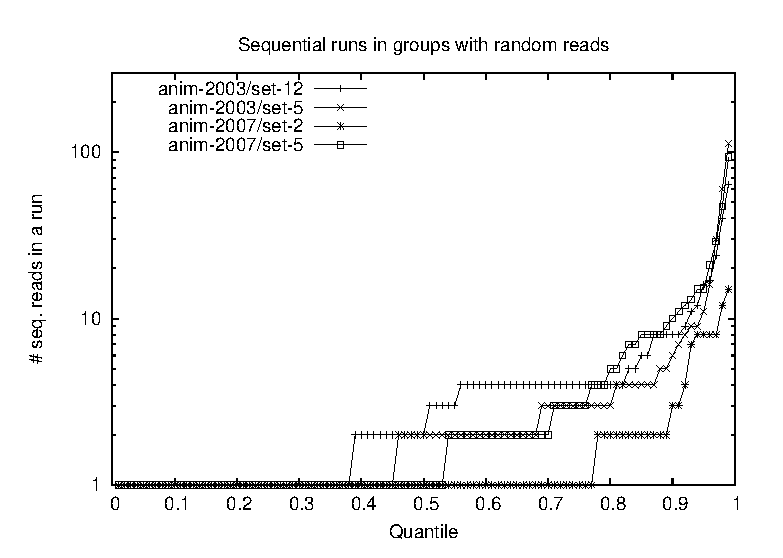
\epsfig{width=2.1in, angle=0, file=graphs/seq-in-random-seq-count.ps}
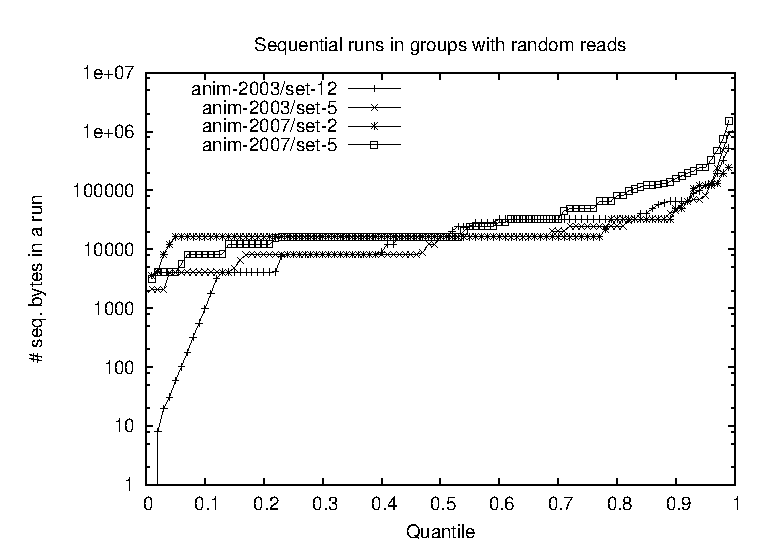
\epsfig{width=3.2in, angle=0, file=graphs/seq-in-random-seq-bytes.ps}
\vspace{-0.2in}
\caption{Number of reads or sequential bytes in a single group (more than 30s gap between I/Os); }
\label{fig:seq-analysis}
\end{figure}


Sequentiality is one of the most important properties for storage
systems because disks are much more efficient when handling sequential
data accesses.  Prior work has presented
various methods for calculating sequentiality.  Both
Ellard~\cite{EllardFast03} and Leung~\cite{LeungUsenix08} split accesses
into groups and calculate the sequentiality within the group.  Ellard
emulates opens and closes by looking for 30s groups in the access
pattern.  Ellard tolerates small gaps in the request stream as
sequential, e.g. an I/O of 7KiB at offset 0 followed by an I/O of 8KiB at
offset 8KiB would be considered sequential.  

Ellard also reorders I/Os
to deal with client-side reordering. In particular, Ellard looks
forward a constant amount from the request time to find I/Os that
could make the access pattern more sequential.  This constant was
determined empirically.  Leung treats the first I/O after an open as
sequential, essentially assuming that the server will prefetch the
first few bytes in the file or that the file is contiguous with the
directory entry as with immediate files~\cite{Mullender84ImmediateFiles}.  
For NFS, the server may not see a lookup before a read, depending on whether
the client has used readdir+ to get the filehandle instead of a lookup.

We determine sequentiality by reordering within temporally overlapping
requests. Given two I/Os, A and B, if the request-reply intervals
overlap, then we are willing to reorder the requests to improve
estimated sequentiality.  We believe this is a better model because
the NFS server could reorder those I/Os.  In practice,
Figure~\ref{fig:seq-bytes-compare} shows that for our traces this
reordering makes little difference.  Allowing reordering an additional
10ms beyond the reply of I/O A slightly increases the sequentiality,
but generally not much more than just for overlapping requests.

We also decide on whether the first I/O is sequential or random based
on additional I/Os.  If the second I/O (after any reordering) is
sequential to the first one, than the first I/O is sequential,
otherwise it is random.  If there is only one I/O to a particular
file, then we consider the I/O to be random since the NFS server would
have to reposition to that file to start the read.  

Given our small file sizes, it turns out that most accesses count as
random because they read the entire file in a single I/O.  We can see
this in Figure~\ref{fig:seq-analysis}(a), which shows the number of
reads in a group.  Most groups are single I/O groups (70-90\% in the
2007 traces).  We see about twice as many I/Os in the 2003 traces,
because the I/Os in the 2003 traces are only 8KiB, rather than 16KiB.

Sequential runs within a random group are more
interesting.  Figure~\ref{fig:seq-analysis}(b) shows the number of
bytes accessed in sequential runs within a
random group.  We can see that if we start accessing a file at random,
most (50-80\%) of the time we will do single or double I/O accesses (8-32KiB).
However we also get some extended runs within a
random group, although 99\% of the runs are less than 1MiB.

% select dataset,operation, max(mean_operations_per_second) from xnfs_hostinfo_rates where group_seconds = 1 and host is null and direction = 'send' and operation is not null and op_dir is null and mean_operations_per_second > 300 group by dataset,operation order by operation
% --> access, fsstat, getattr, lookup, read, write 

\begin{figure}
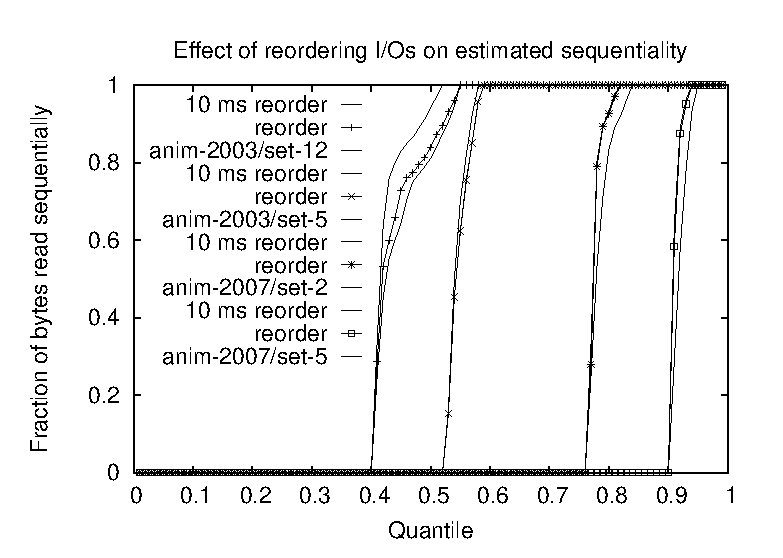
\epsfig{width=3.2in, angle=0, file=graphs/seq-bytes-compare.ps}
\vspace{-0.1in}
\caption{Each line group shows host estimated sequentiality was affected by allowing, in order: 
reordering of I/Os within 10ms of the
reply, reordering within the request-reply window, or no reordering.
The small horizontal change shows that reordering 
this workload has a negligible effect on sequentiality.}
\label{fig:seq-bytes-compare}
\end{figure}



% LocalWords:  perf op GHz Opterons MiB anim burstiness Mbps kpps mbps Gb Gbit
% LocalWords:  Leung bursty Mbit filesystem getattrs ops NFSv KiB readdirplus
% LocalWords:  filehandle getattr  IP RPC endian nfsdump RPCs RPC's MEMS seq
% LocalWords:  Ellard
% LocalWords:  prefetch readdir xnfs hostinfo dir fsstat
